\documentclass[11pt]{article} % do not change this line
\input{BigDataStyle.txt}      % do not change this line
\usepackage{amsmath,amsfonts,amssymb,amsthm,latexsym,graphicx}
\usepackage{lipsum}

\emergencystretch=5mm
\tolerance=400
\allowdisplaybreaks[4]

\graphicspath{ {./images/} }

\theoremstyle{plain}
\newtheorem{theorem}{Theorem}[section]
\newtheorem{proposition}[theorem]{Proposition}
\newtheorem{corollary}[theorem]{Corollary}
\newtheorem{lemma}[theorem]{Lemma}
\newtheorem{problem}[theorem]{Problem}

\theoremstyle{definition}
\newtheorem*{remark}{Remark}

\title{Deep Learning}
\author{Michael Harrison}

\newcommand{\Programme}{Machine Learning}
% Computational Finance students: uncomment the next line
%\twodepartmentstrue

\begin{document}
\maketitle

\declaration

\begin{abstract}
  This dissertation covers a bunch of stuff!
\end{abstract}

\listoffigures
\newpage

\section{Section one}

This is a sample section.

\section{Section two}

An example of a reference:
\cite{hastie/etal:2009}.

\section{Section three}

Here's another example of a reference:
\cite{MURA2017}

\newpage
\section{Section four}
\lipsum

\newpage
\section{Section five}
\subsection{Subsection one}
This is subsection one

\subsection{Subsection two}
\subsubsection{Subsubsection one}
This is sub-sub-section one of subsection two.

\newpage
\section{Image Test}

\begin{figure}[!ht]
  \caption{Example X-Ray Image}
  \label{fig:xray1}
  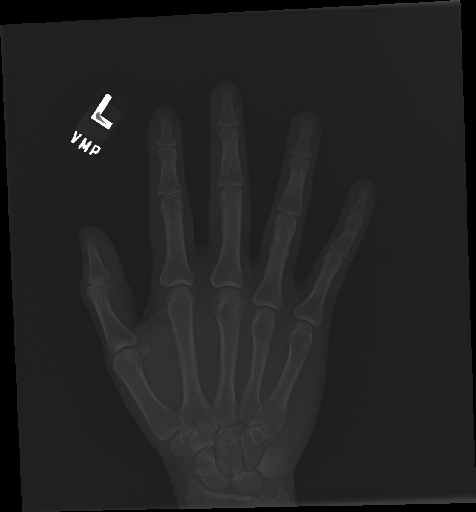
\includegraphics[width=\textwidth, height=8cm]{image1}
  \centering
\end{figure}

\begin{figure}[!ht]
  \caption{Another example X-Ray Image}
  \label{fig:xray2}
  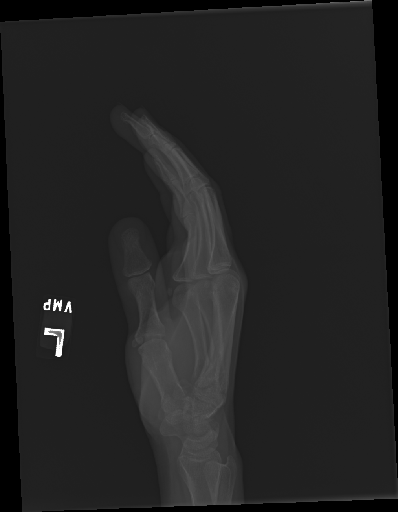
\includegraphics[width=\textwidth, height=8cm]{image2}
  \centering
\end{figure}

As can be seen in \textbf{Figure \ref{fig:xray1}}, the x-ray is of a hand. A side-profile of the hand from the same study can be seen in \textbf{Figure \ref{fig:xray2}}.

\clearpage
\bibliographystyle{plain}
\bibliography{bibliography}
\end{document}
